\chapter{Neural networks expressivity}



\section{Perceptron}

Single neuron that defines a binary threshold through a hyperplane:
\[
    \begin{cases}
        1 & \sum_{i} w_i x_i + b \geq 0 \\
        0 & \text{otherwise}
    \end{cases}    
\]

\begin{description}
    \item[Expressivity] \marginnote{Perceptron expressivity}
        A perceptron can represent a NAND gate but not a XOR gate.
        \begin{center}
            \begin{minipage}{.2\textwidth}
                \centering
                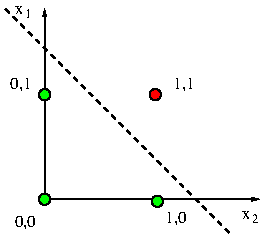
\includegraphics[width=\textwidth]{img/_perceptron_nand.pdf}
                \tiny NAND
            \end{minipage}
            \begin{minipage}{.2\textwidth}
                \centering
                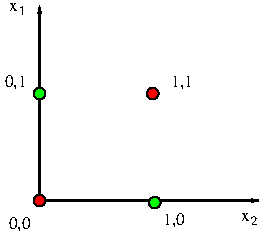
\includegraphics[width=\textwidth]{img/_xor.pdf}
                \tiny XOR
            \end{minipage}
        \end{center}

        \begin{remark}
            Even if NAND is logically complete, the strict definition of a perceptron is not a composition of them.
        \end{remark}
\end{description}



\section{Multi-layer perceptron}

Composition of perceptrons.

\begin{descriptionlist}
    \item[Shallow neural network] \marginnote{Shallow NN}
        Neural network with one hidden layer.

    \item[Deep neural network] \marginnote{Deep NN}
        Neural network with more than one hidden layer.
\end{descriptionlist}

\begin{description}
    \item[Expressivity] \marginnote{Multi-layer perceptron expressivity}
        Shallow neural networks allow to approximate any continuous function 
        \[ f: \mathbb{R} \rightarrow [0, 1] \]

        \begin{remark}
            Still, deep neural networks allow to use less neural units.
        \end{remark}
\end{description}


\subsection{Parameters}

The number of parameters of a layer is given by:
\[ S_\text{in} \cdot S_\text{out} + S_\text{out} \]
where:
\begin{itemize}
    \item $S_\text{in}$ is the dimension of the input of the layer.
    \item $S_\text{out}$ is the dimension of the output of the layer.
\end{itemize}

Therefore, the number of FLOPS is of order:
\[ S_\text{in} \cdot S_\text{out} \]